\begin{figure*}
	\centering
	\vspace{0.5cm}
	\includegraphics{figures/fancy-figure.pdf}
 \caption{ This visualisation shows two epochs at once, simultaneously
 showing the initial conditions (in blue and red) and the final simulation
 volume at redshift $z=0$ in white/grey. The blue and red show the positions
 of the gas and dark matter (respectively) \emph{in the initial conditions}
 for particles that reside in selected haloes at redshift $z=0$. The overlaid
 white/grey map shows the dark matter at redshift $z=0$ to enable comparisons
 between the initial and final comoving positions for various bound
 structures. For each selected halo, the dashed black circles show their
 virial radii as defined in \ref{sec:simba}. For some haloes in crowded
 regions, we have overlaid a circle and arrows showing which blob of dark
 matter and gas in the initial conditions collapses to form this halo.
 Finally, for each halo we show a small bar chart showing their final
 Lagrangian make-up, as described later in the text. This figure illustrates
 the significant differences in origin between the gas (blue) and dark matter
 (red) for these selected haloes of various masses. We also see how the
 environment of each halo changes its Lagrangian make-up. In particular,
 group 431 shows a large baryonic component originating from the Lagrangian
 region of another halo, with this halo entering a small cluster environment
 near the end of the simulation. Note that individual regions are
 colour-mapped separately, i.e. the intensity of colour for a single halo is
 unique to that halo only, as to enable all Lagrangian regions to be seen.
 Without this choice, the structure for the lower mass haloes would be
 completely washed out.}
	\vspace{1cm}
	\label{fig:bigtransferpic}
\end{figure*}


\begin{figure*}
    \centering
    \vspace{1cm}
    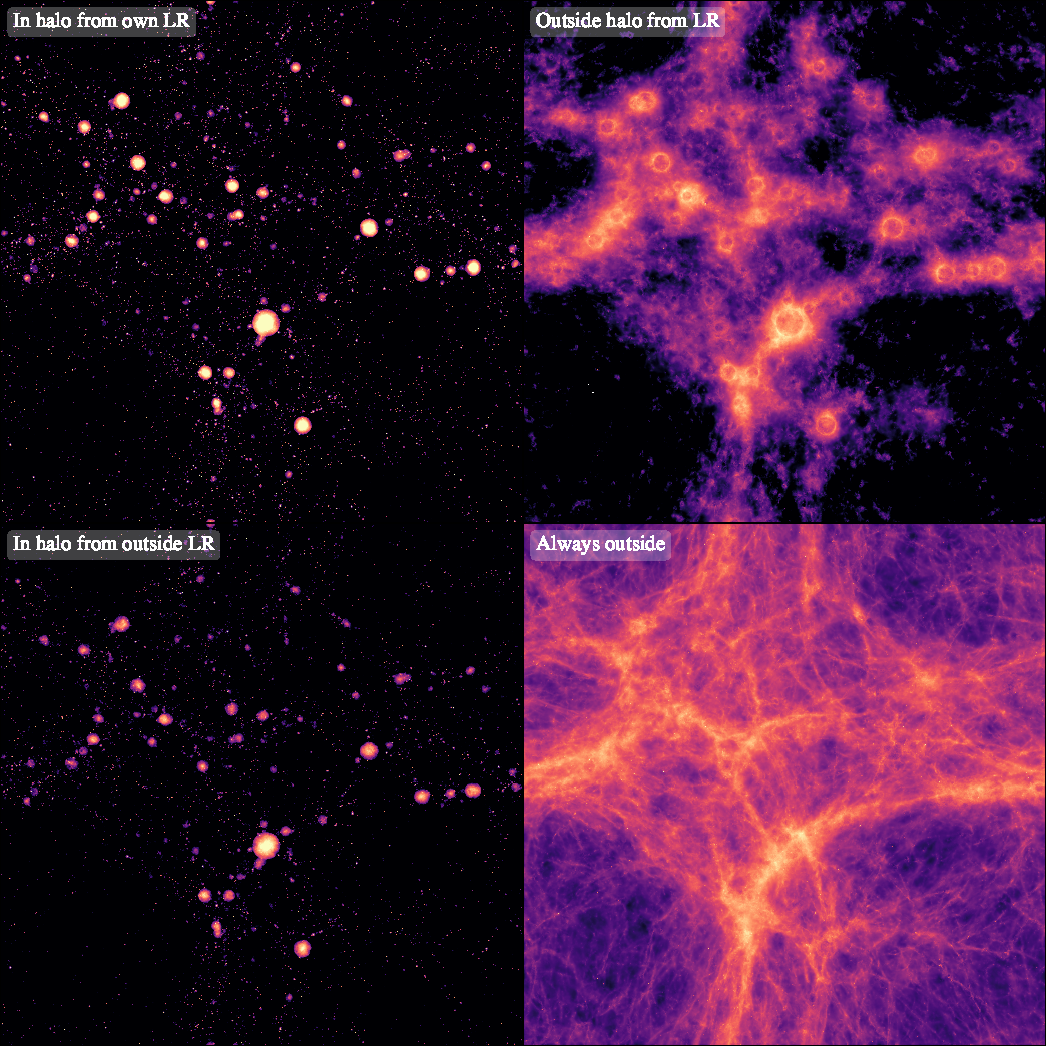
\includegraphics{figures/s50j7kAHF/four_images_magma_AHF.pdf}
    \caption{Gas distribution in the fiducial \simba{} model for the full
    $50\hmpc{}$ volume, split by the following Lagrangian components
    (clockwise, starting from top left): particles that began in Lagrangian
    regions at $z=99$ and have remained in the associated haloes at $z=0$;
    particles that began in Lagrangian regions and ended up outside of the
    destination halo; particles that began outside any Lagrangian region and
    ended up outside any halo; and particles that ended up in a halo but
    originated outside any Lagrangian region. All images are shown with the
    same (logarithmic) colour-map and normalisation and taking their linear
    sum would reproduce the full gas distribution at $z=0$. Gas particles
    that began in Lagrangian regions but ended up outside of haloes (top
    right) show a striking similarity to the distribution of gas with the
    33\% highest spread distance shown in Fig.~\ref{fig:bigdistanceimage}.
    As expected, particles that began outside of Lagrangian regions and
    remained outside of haloes (bottom right) trace the filaments and voids.}
    \vspace{1cm}
    \label{fig:lrtransfer}
\end{figure*}

\section{Lagrangian baryon transfer}
\label{sec:transfer}

We have explored the relative motion of dark matter and baryons using a
particle-level metric, showing that AGN jets in the \simba{} cosmological
simulations can spread baryons up to $12\hmpc{}$ relative to the neighbouring
dark matter. In this section, we consider the movement of baryons relative to
dark matter haloes and their corresponding Lagrangian regions. The definitions of
haloes and Lagrangian regions used here are described in \S \ref{sec:simba}.

\subsection{The different origins of baryons and dark matter in haloes}

Fig. \ref{fig:bigtransferpic} illustrates the mixed origins of the gas and
dark matter components in bound structures at $z=0$ by showing simultaneously
the initial and final states of the simulation. A common trend for all haloes
is a shell of gas around the main dark matter component in the initial
conditions, showing that gas in general is able to collapse further (due to
cooling and other processes) than the dark matter, which is unable to lose
angular momentum as efficiently. This is consistent with the larger values of
the spread metric for gas in haloes relative to the dark matter in haloes, as
shown in Fig. \ref{fig:distbaryon}.

The origin of the dark matter in the initial conditions corresponds
exactly to our definition of Lagrangian region for that component in \S
\ref{sec:simba}. These Lagrangian regions have very complex shapes, with them
becoming more complex with lower halo mass (as objects become less powerful
attractors) and increasing amounts of transfer (see below). Larger haloes tend
to have more spherical Lagrangian regions, as can be seen with the largest
halo in the box (Group 0) in Fig. \ref{fig:bigtransferpic}. These
non-spherical shapes are why we chose to identify our Lagrangian regions for
gas in the way that we did (i.e. through neighbour searching, rather than
through a fixed 3D aperture), as anything else would leave us unable to
capture the surprisingly intricate structure that is at play here.

There are many possible reasons for the complex shapes that we see here.
Consider a simple case where we have one `main' halo, and a satellite that is
being accreted. This has several possible fates. As the satellite begins to
fall into the main halo, its gas may be shocked and halted in the CGM, with
the dark matter continuing to fall in, separating baryonic and dark
component. The gas may then be expelled by a feedback event, simply rise out
of the halo boundary due to its buoyancy, or cool and join the dark matter in
the centre of the halo. In the case where both the dark matter and gas fall
into the central, there is yet another chance for them to be separated, with
the gas being subject to feedback events. Once the gas has been removed from
the halo, it is free to be `picked up` by other passing haloes, or lie
outside of the halo in the IGM. The other possibility for the fate of this
substructure is the dark matter failing to accrete onto the central. In this
case, the dark matter continues moving out into the IGM, with the gas being
shocked and captured by the main halo. In this case, the gas would be
classified as originating outside any Lagrangian region.

\subsection{Computing transfer between Lagrangian regions}

Given the definitions of haloes and Lagrangian regions in
\S \ref{sec:simba}, it is possible to classify every particle in the
simulation according to their Lagrangian ID and Halo ID (if any) in the
initial and final conditions. The algorithm is as follows:

\begin{enumerate}
	\item ID match all particles between the initial and final conditions, including
	      star particles (these are matched to their gas progenitor). Black holes are ignored in this analysis since globally they represent a minimal amount of mass.

	\item Every particle at $z=0$ has several possible final states and origins, based on its halo ID ($i$) and Lagrangian region ID ($j$):
	      \begin{itemize}
	            \item Particle resides in  halo ($i \neq -1$)
	            \begin{itemize}
	           		\item Particle originated in the same Lagrangian region, $j = i$
	           		\item Particle originated outside any Lagrangian region, $j \equiv -1$
	           		\item Particle originated in some other Lagrangian region, $j \neq i$
	            \end{itemize}
	            \item Particle resides outside of any halo ($i \equiv -1$)
	            \begin{itemize}
	            	\item Particle originated outside any Lagrangian region, $j = i$
	            	\item Particle originated in some Lagrangian region, $j \neq i$
	            \end{itemize}
	      \end{itemize}
	      
	\item For every halo and Lagrangian region, the mass originating from each
	      of the above components is computed and stored.
\end{enumerate}

A visualisation of this particle classification scheme is shown in
Fig.~\ref{fig:lrtransfer}, where we split the gas distribution in the
\simba{} $50\hmpc{}$ box into the four main Lagrangian components that we
consider in the remainder of this paper. Considering each panel clockwise
from the top left, we select first the gas that is in the same halo at
redshift $z=0$ as the Lagrangian region that it originated in. As expected,
we see a population of spherical shapes corresponding to every halo in the
box, with their sizes corresponding to $R_{\rm vir}$ as defined by AHF. The
centers of haloes, where the gas is densest, are the brightest.

In the top right panel we have the gas that is outside any halo at $z=0$, but
is assigned to a Lagrangian region at $z=99$; this is the gas that should
have ended up in haloes by the end of the simulation if the baryonic matter
was also collisionless. We see that this component traces gas primarily
around massive haloes, resembling the large-scale bubbles that the AGN jets
power in \simba{} \citep{Dave2019}. Note that some of this gas piles up just
outside of haloes owing to the somewhat arbitrary boundary defined by the
virial radius of haloes. This gas resides primarily in filaments, with some
reaching out into the voids.

In the bottom right panel, we visualise the gas that begun outside any
Lagrangian region and resides outside any halo at redshift $z=0$. This gas
traces the majority of the filamentary structure, and shows all of the
structure in the voids. 

Finally, in the bottom left panel, we have the gas that is in haloes at $z=0$
but originated from outside any Lagrangian region. As expected, this shows a
very similar structure (albeit less bright) to the gas that resides in its
own halo (top left), but this component originates from regions where the
dark matter now resides outside of haloes. This gas is likely dragged into
these bound structures by cooling flows, while the dark matter
is not able to lose angular momentum quickly enough to assemble by $z=0$.

\subsection{Transfer in a non-radiative Model}

\begin{figure}
	\centering
	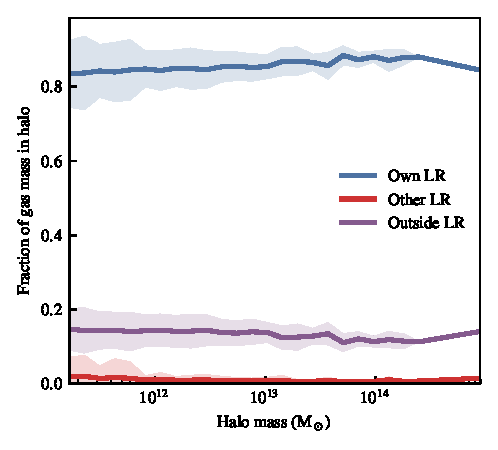
\includegraphics[width=\columnwidth]{figures/s50gadget/component_fraction_vs_halo_mass_gas.pdf}
	\vspace{-0.7cm}
 \caption{ The fraction of baryonic mass originating from each Lagrangian
 component in the non-radiative model (i.e. without sub-grid physics) is
 shown as a function of redshift $z=0$ halo mass. The gas particles are
 binned by their origin, with the baryons originating from their own
 Lagrangian region shown in blue, the Lagrangian region of other haloes
 (red), and outside of any Lagrangian region (purple). Shaded regions show
 the $1\sigma$ scatter in a given bin, which is given by one standard
 deviation of variation. The lines represent the mean value within each bin.
 Approximately 85\% of the baryonic mass of a given halo originates from its
 own Lagrangian region, showing very little transfer of baryons from either
 outside or from another Lagrangian region. This is provided for comparison
 to the full model result in Fig. \ref{fig:maintransferresult}.}
	\label{fig:nonradiativetransfer}
\end{figure}

\begin{figure*}
	\centering
	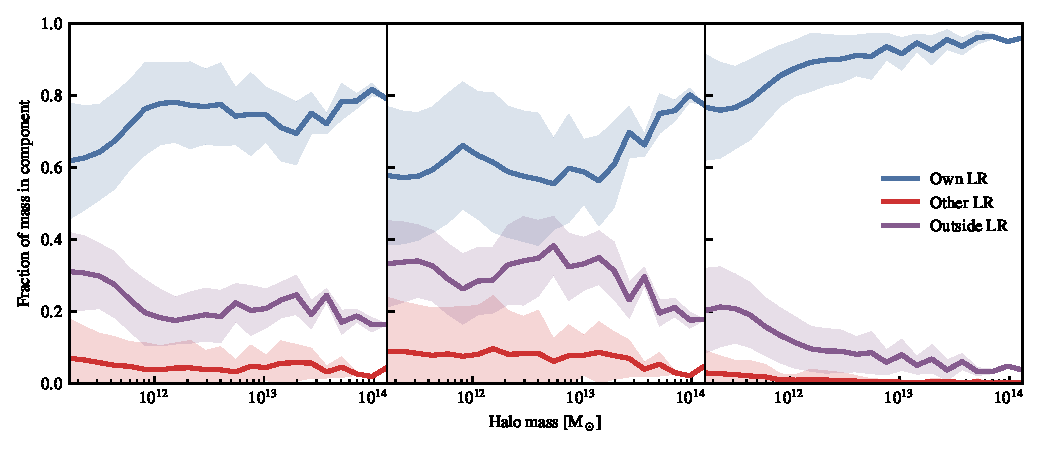
\includegraphics{figures/s50j7kAHF/component_fraction_mixed.pdf}
	\vspace{-0.7cm}
	\caption{
  The fraction of baryonic mass in haloes at $z=0$ originating from their own
  Lagrangian region (blue), the Lagrangian region of other haloes (red), and
  outside of any Lagrangian region (purple), shown as a function of $z=0$
  halo mass for the fiducial \simba{} model. We consider all baryons in
  haloes (left) as well as their gas (center) and stellar (right) components
  separately.
	}
	\label{fig:maintransferresult}
\end{figure*}

Before considering the numerical results of the full model, we first present
the non-radiative simulation as a null model to investigate the effects of
hydrodynamics alone. In this case, we run the simulation without cooling,
star formation, or feedback, only including hydrodynamics, cosmology, and
gravity. In Fig. \ref{fig:nonradiativetransfer} we present the fraction of
baryonic mass for each halo contributed from each Lagrangian component, as a
function of halo mass. The blue line shows the fraction of mass in each halo
from its own Lagrangian region (top left in Fig. \ref{fig:lrtransfer}), the
red shows transfer into a halo from another Lagrangian region (top right in
Fig. \ref{fig:lrtransfer}), and the purple line shows the fraction of
baryonic mass from outside any Lagrangian region (bottom left in Fig.
\ref{fig:lrtransfer}). There is no dependence on halo mass (as the simulation is
effectively scale-free above some resolution limit), and apart from some
small level of transfer from outside any Lagrangian region, the baryonic mass
in each halo consists of that which originated in its own Lagrangian region.
This difference is likely to be caused caused by gas that piles up on the
outside of each halo due to accretion shocks while the collisionless dark
matter is stripped by passing straight through or around the bound structure.

\subsection{Transfer \emph{into} haloes}
\label{sec:transferinto}

Moving on to the full \simba{} model, we consider again the fractions of
baryonic mass as a function of halo mass, split by Lagrangian component. Fig.
\ref{fig:maintransferresult} shows three panels: the left panel shows all
baryons, the centre shows only gas, and the right panel shows the
contribution from only the stars. The lines are coloured the same as the
non-radiative model shown in Fig. \ref{fig:nonradiativetransfer}. Now that we
have introduced scale into the simulation through density-dependent energy
injection mechanisms, these components scale with halo mass. The general
trend is that for an increasing halo mass, a Lagrangian region is able to
hold on to more of the original baryonic mass, with this flattening off
around $M_H = 10^{12} \msolar$. For a given halo, significantly more of the
gaseous mass originates outside the original Lagrangian region as compared to
the stellar mass ($\sim 40 \%$ versus $\sim 10 \%$). The transfer between
haloes is at around the $\sim 10\%$ baryonic mass level, with this transfer
predominantly originating from the gaseous component, as compared to the
stellar component. This combines nicely with the distance metrics shown in \S
\ref{sec:feedbackmetrics}, which showed that the dark matter and stars have
very similar dynamics and hence should be similarly well bound.

This transfer into, and between, Lagrangian regions can have several physical
origins. The first, as shown in the non-radiative run, is caused by the
collisional dynamics of the gas preventing gas from following the dark matter
in all cases. We see that this can account for up to 15\% of the baryonic
mass of a bound structure at redshift $z=0$ originating from a different
region than the dark matter, but this could not account for any
\emph{inter-Lagrangian} region transfer.

The galaxy formation sub-grid model clearly has a significant effect on the
baryonic make-up of haloes at redshift $z=0$. The fraction of mass from
outside any Lagrangian region have increased to 20-40\%. This increase is
explained by the inclusion of sub-grid cooling and feedback processes, with
particles now able to form cool accretion flows that can lose angular
momentum at a much higher rate than the dark matter component is able to.

Around 10\% of the baryonic mass of haloes is now made up of gas that has
experienced inter-Lagrangian transfer. It is important to recall that this is transfer
between bound structures at redshift $z=0$, and that it only takes into account
the initial and final conditions of the simulation; we do not know the complete history
of these particles.

The transfer between haloes has several possible sources: stripped gas from
nearby galaxies that are still classified as their own bound structures at
redshift $z=0$, gas that has been expelled from galaxies through stellar
winds or AGN feedback and re-captured by a halo, and spurious transfer in the
initial conditions due to the way that we have classified our Lagrangian
regions. With the non-radiative simulation showing zero transfer between
haloes, and there being little transfer before redshift $z=2$ in the fiducial
model, we believe that the contribution from this component is likely very
small. When repeating this analysis with the \nojet{} run, the
inter-Lagrangian transfer is reduced by a small amount, but still remains at
the 10\% level. If this transfer is powered by feedback events it must be
dominated by the expulsion (or preventative feedback) from stellar winds and
the residual thermal AGN feedback.

A given mass bin contains haloes that entertain a range of 10x in transfer,
which is likely dependent on environment as shown in Fig.
\ref{fig:bigtransferpic}. Future work should investigate in more detail
the physical mechanisms driving the scatter in these relations.

The results above $10^{13} \msolar{}$ are quite uncertain, as there are
very few haloes above this mass present in the box (less than 50), with the
small scatter being misleading. It is also important to note that the shaded
regions in Fig. \ref{fig:maintransferresult} represent the $1\sigma$
scatter in a given bin and explicitly do \emph{not} include any errors that
would occur from a finite sampling of haloes or halo assembly bias.

\subsection{Transfer \emph{out} of Lagrangian Regions}

\begin{figure}
	\centering
	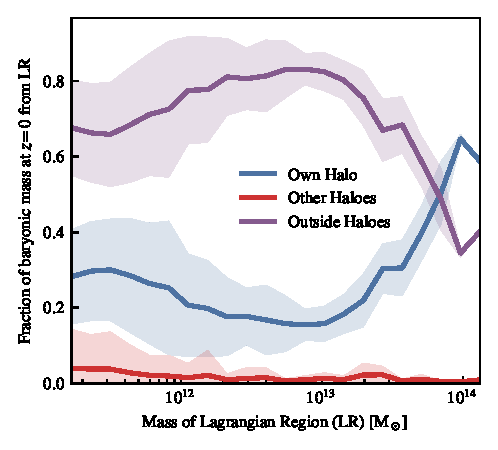
\includegraphics{figures/s50j7kAHF/inverse_component_fraction.pdf}
	\vspace{-0.7cm}
	\caption{The fate of gas that begins in Lagrangian regions, as a function of
	initial Lagrangian region mass. The blue line shows the fraction of baryons
	that reside in the halo that defines the Lagrangian region at redshift $z=0$,
	the red line shows the the fraction of baryons that lie in a different halo,
	and the purple line shows the baryons that lie outside of any halo at redshift
	$z=0$. All but the most massive objects in the box struggle to retain more than
	20\% of their baryons due to various factors, see the text for details.}
	\label{fig:transferoutoflrs}
\end{figure}


\begin{figure}
	\centering
	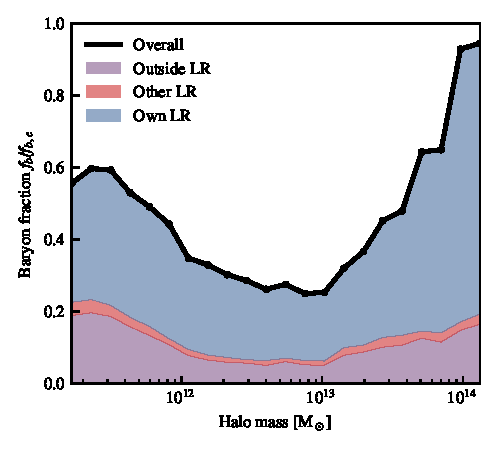
\includegraphics{figures/s50j7kAHF/baryon_fraction_breakdown.pdf}
	\vspace{-0.7cm}
	\caption{The baryon fraction $f_b$ relative to the cosmic baryon fraction
	$f_{b, c}$ shown as a function of halo mass. The coloured bands show the
	contributions to the baryon fraction from various Lagrangian components.}
	\label{fig:baryonfraction}
\end{figure}

Let us now move on to consider the fates of baryons that begin their lives in
Lagrangian regions. This material has three possible fates, as shown in Fig.
\ref{fig:transferoutoflrs} it can: end up in the same halo as the dark matter
from that Lagrangian region (blue line); end up in another halo (red line),
or outside of any halo in the IGM (purple line). Here, we plot the results as
a function of their Lagrangian region mass (this is the sum of the baryons
and dark matter contained within that Lagrangian region). This is somewhat
higher than the eventual halo mass due to the baryon fractions of redshift
$z=0$ haloes being below the cosmic mean. We see that, below a halo mass of
$10^{13}\msolar{}$, only around 20\% of the baryons initially present in the
Lagrangian region make it in to the halo at $z=0$. Only above a halo mass of
$10^{14}\msolar{}$ do haloes become strong enough attractors to retain the
majority of their baryons. This latter result is somewhat uncertain, however,
due to the very small number of these very large haloes present in our
$50\hmpc{}$ box. On top of this initial structure, we see that there is a dip
in the retained fraction of baryons between $10^{12}$ and $10^{13}\msolar{}$.
We speculate that this is due to the increased efficiency of AGN feedback in
haloes in this mass range, allowing for more of the dense gas in central
objects to be expelled, however making a direct connection would require 
significant investigation out of the scope of this work. It is worth noting that
without the AGN jets (i.e. in the \nojet{} run), the baryon fraction of haloes
in this mass range is approximately $f_b / f_{b,c} = 1$.

Finally, we see that the fraction of baryons transferred out of the Lagrangian
region into other haloes drops of slowly with halo mass. A larger cosmological
volume with more objects is required for a full study here, but these trends
point towards inter-Lagrangian transfer being fuelled by accretion of gas
that is either expelled or stripped from lower mass haloes by higher mass
objects. This appears consistent with the results in \S \ref{sec:transferinto},
where we found that little transfer between objects occurs before redshift
$z=2$. A plausible physical scenario is that early feedback leading up to
redshift $z=2$, where star formation (and hence stellar feedback) peaks,
expels significant quantities of gas from lower mass haloes that can then be
swept up at later times from the IGM by all objects. Higher mass haloes at this
redshift may have a strong enough gravitational potential to enable their stellar
winds to be more efficiently recycled, preventing them from being sources
of inter-Lagrangian transfer.

The combination of the baryons that are retained by haloes (Fig.
\ref{fig:transferoutoflrs}) and the baryons that they manage to accrete from
sources outside their Lagrangian region (Fig. \ref{fig:maintransferresult})
is seen in the baryon fraction of haloes, shown in Fig.
\ref{fig:baryonfraction} here split by Lagrangian component. Here, we split
the overall baryon fraction (relative to the cosmic mean) into three
Lagrangian components, coloured by the baryons from the haloes own Lagrangian
region (blue), other Lagrangian regions (red), and from outside any
Lagrangian region (purple). In general, we see that there is a trough in the
baryon fractions of haloes with a mass between $10^{12}$ and
$10^{13}\msolar{}$, with the baryon fraction reaching the cosmic mean for the
largest objects in the box (with a halo mass of $10^{14}\msolar{}$). The
baryon fraction returning to $f_b = 1$ for these very large haloes is not
caused by these haloes retaining all of their Lagrangian gas, however; it is
caused by a complex interplay between their accretion from outside, from
other Lagrangian regions, and from the significant component that originates
outside of any Lagrangian region. These objects are clearly able to mix
outside of their halo boundaries, swapping gas with the IGM, as has been
shown in several studies \cite{Mansfield2017, Diemer2017} through `splashback'.

The dip in baryon fraction between $10^{12}$ and $10^{13}\msolar{}$ in halo
mass corresponds to the dip in retained baryons in a similar mass range in
Fig. \ref{fig:transferoutoflrs}. However, within this mass range, it appears
that the fraction of baryons originating from outside the Lagrangian region is
more significantly affected (reduced by 50\% as opposed to 20\%). This points
to a more complex accretion history for these objects, with a mixture of
ejective (in general reducing the amount of retained baryons) and preventative
feedback (in general reducing the amount of baryons from outside of the
corresponding Lagrangian region) shaping their baryonic content.

